\documentclass{article}
\usepackage[utf8]{inputenc}
\usepackage[T1]{fontenc}
\usepackage[english]{babel}
\usepackage{graphicx}
\usepackage{physics}
\usepackage{calrsfs}
\usepackage{mathalpha}
\usepackage{amssymb}
\usepackage{amsfonts}
\usepackage{amsmath}
\usepackage{fixltx2e}
\usepackage{float}
\usepackage{caption}
\usepackage{hyperref}

\title{2021-03-30}
\author{}
\date{March 2021}

\graphicspath{{images/}}

\begin{document}

\maketitle

\section{Review of the Galois multiplaction}
In order to implement the GCM we need to perform Galois Field Multiplications.

\begin{figure}[H]
    \centering
    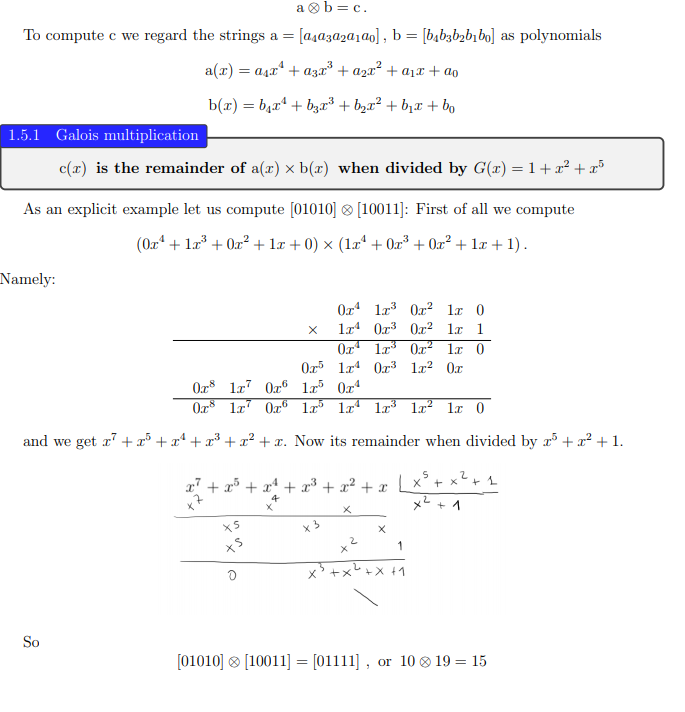
\includegraphics[scale=0.50]{1.png}
\end{figure}
\section{Isomorphism}
an isomorphism is a structure-preserving mapping between two structures of the same type that can be reversed by an inverse mapping.
Why isomorphism is important in this context and how to get it?
The irreducible polynomial is defined as a parameter in the Galois Multiplication, said polynomial is not unique inside the same Galois Field, so by using different irreducible polynomials inside the same Galois Field we define different Galois Groups each one related to the other one for isomorphism.
Let's suppose to do   $$ a \oplus b = c $$ where $$ G(x) $$ is the irreducible polynomial.
If we consider another irreducible polynomial $ H(x) $ and perform the Galois Multiplication $$ a \oplus b = d $$ such that $$ F(a) \oplus F(b) = F(a\oplus b) $$ where F is an invertible function which maps a set of bits into a different Group of the same Galois Field. By applying the function twice on a string of bits we would obtain the same string again.
F is a way to map a sequence of bit into another one by means of isomorphism.
In order to implement this mapping an invertible matrix P is used. The last row of P is all zeros except the bit in the last coloumn, the second to last row consists of a polynomial $ \alpha (x) $ such that if evaluated in $ G ( \alpha (x) ) $ is 0, said polynomial $  \alpha (x) $ is also called root of G.
Let's suppose we use G as irreducible polynomial for this multiplication $ a \oplus b = c $, now let's suppose we want to know the result of the same operation but we use $  \alpha (x) $  as irreducible polynomial. Since we already know the result c, instead of performing again the multiplication it is enough to multiply the array of bits c by the matrix P.

This is convenient since the computation of the matrix can be done just one time and avoid us the multiplication of each of the factors again if we want to have the result corresponding to a different group of another irreducible polynomial for the same Galois Field.
\section{GCM}
The Galois Counter Mode (GCM) is an encryption mode which also computes a
message authentication code (MAC). A MAC provides a cryptographic checksum that is computed by the sender, Alice, and appended to the message. Bob also
computes a MAC from the message and checks whether his MAC is the same as
the one computed by Alice. This way, Bob can make sure that (1) the message was
really created by Alice and (2) that nobody tampered with the ciphertext during
transmission. These two properties are called message authentication and integrity,
respectively. Much more about MACs is found in Chap. 12. We presented a slightly
simplified version of the GCM mode in the following.
GCM protects the confidentiality of the plaintext x by using an encryption in
counter mode. Additionally, GCM protects not only the authenticity of the plaintext
x but also the authenticity of a string AAD called additional authenticated data.
This authenticated data is, in contrast to the plaintext, left in clear in this mode of
operation. In practice, the string AAD might include addresses and parameters in a
network protocol.
The GCM consists of an underlying block cipher and a Galois field multiplier
with which the two GCM functions authenticated encryption and authenticated decryption are realized. The cipher needs to have a block size of 128 bits such as AES.
On the sender side, GCM encrypts data using the Counter Mode (CTR) followed by
the computation of a MAC value. For encryption, first an initial counter is derived
from an IV and a serial number. Then the initial counter value is incremented, and
this value is encrypted and XORed with the first plaintext block. For subsequent
plaintexts, the counter is incremented and then encrypted. Note that the underlying
block cipher is only used in encryption mode. GCM allows for precomputation of
the block cipher function if the initialization vector is known ahead of time.
For authentication, GCM performs a chained Galois field multiplication. For every plaintext x i an intermediate authentication parameter g i is derived. g i is computed as the XOR sum of the current ciphertext y i and g i , and multiplied by the
constant H.
The value H is a hash subkey which is generated by encryption of the
all-zero input with the block cipher. All multiplications are in the 128-bit Galois
field GF(2 128 ) with the irreducible polynomial P(x) = x 128 + x 7 + x 2 + x + 1. Since
only one multiplication is required per block cipher encryption, the GCM mode adds
very little computational overhead to the encryption.
\begin{figure}[H]
    \centering
    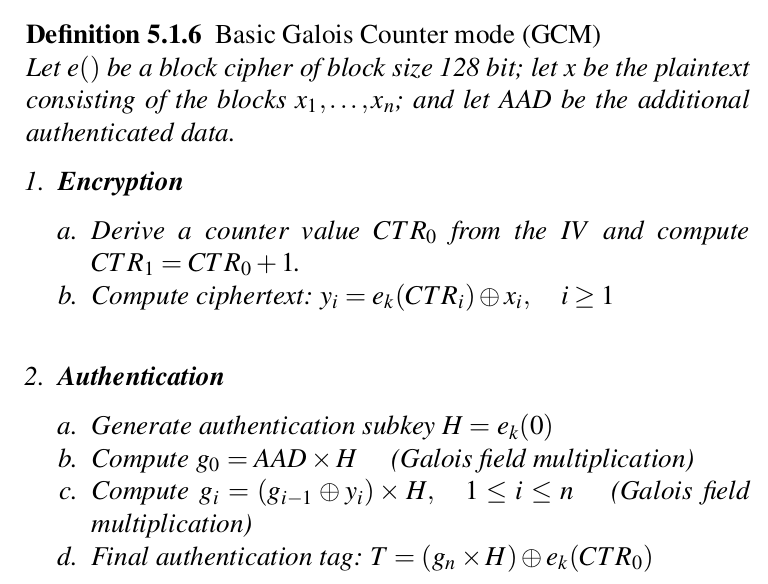
\includegraphics[scale=0.35]{2.png}
\end{figure}
\begin{figure}[H]
    \centering
    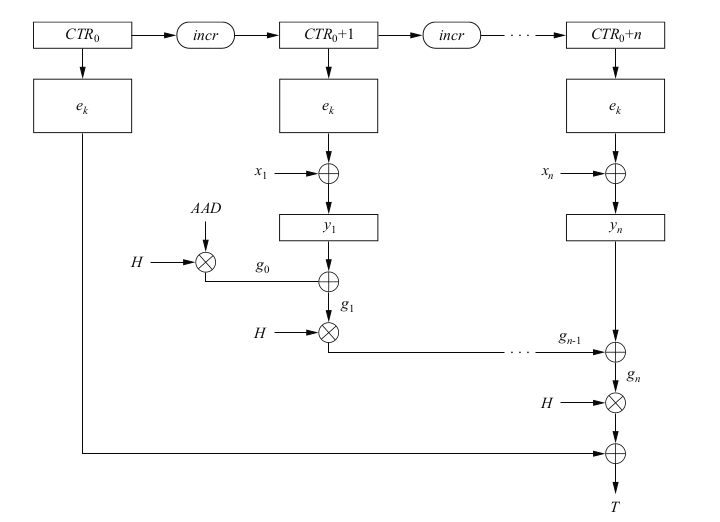
\includegraphics[scale=0.35]{3.png}
\end{figure}
The receiver of the packet [(y 1 , . . . , y n ), T, ADD] decrypts the ciphertext by also
applying the Counter mode. To check the authenticity of the data, the receiver also
computes an authentication tag T using the received ciphertext and ADD as input.
He employs exactly the same steps as the sender. If T and T match, the receiver is
assured that the cipertext (and ADD) were not manipulated in transit and that only
the sender could have generated the message.
\end{document}
